
\documentclass{ifacconf}
\newcounter{part}
\counterwithin*{section}{part}
\usepackage{graphicx}      % include this line if your document contains figures
\usepackage{natbib}        % required for bibliography
%===============================================================================
% Proof Env
\makeatletter
\DeclareRobustCommand{\qed}{%
  \ifmmode % if math mode, assume display: omit penalty etc.
  \else \leavevmode\unskip\penalty9999 \hbox{}\nobreak\hfill
  \fi
  \quad\hbox{\qedsymbol}}
\newcommand{\openbox}{\leavevmode
  \hbox to.77778em{%
  \hfil\vrule
  \vbox to.675em{\hrule width.6em\vfil\hrule}%
  \vrule\hfil}}
\newcommand{\qedsymbol}{\openbox}
\newenvironment{proof}[1][\proofname]{\par
  \normalfont
  \topsep6\p@\@plus6\p@ \trivlist
  \item[\hskip\labelsep\itshape
    #1.]\ignorespaces
}{%
  \qed\endtrivlist
}
\newcommand{\proofname}{Proof}
\makeatother
%===============================================================================
\usepackage{xcolor}
\usepackage{scalerel,stackengine,amsmath,amssymb,amsfonts,mathtools,bm}
\usepackage[hyphens]{url}
%\usepackage{hyperref} 
\usepackage[capitalize,noabbrev]{cleveref}
\Crefname{algocf}{Algorithm}{Algorithms}
\crefname{algocf}{Algorithm}{Algorithms}
\crefname{thm}{Assumption}{Assumptions}
\Crefname{thm}{Assumption}{Assumptions}


\usepackage{booktabs}
\usepackage[acronym]{glossaries}

\usepackage[caption=false,font=footnotesize]{subfig}

%\usepackage[backend=biber, style=plain, sorting=none]{biblatex}
%\addbibresource{biblio.bib}
\usepackage[linesnumbered,ruled,boxed,algo2e]{algorithm2e}
\usepackage{pifont}

\usepackage{siunitx}

\newcommand{\cf}{c.\,f. }
\newcommand{\eg}{e.\,g., }
\newcommand{\ie}{i.\,e., }
\newcommand{\linea}[1]{line\:{\footnotesize \textbf{(#1)}}}
\newcommand{\norm}[1]{\left\lVert#1\right\rVert}
\newcommand{\bx}{\bm{x}}
\newcommand\equalhat{\mathrel{\stackon[1.5pt]{=}{\stretchto{%
    \scalerel*[\widthof{=}]{\wedge}{\rule{1ex}{3ex}}}{0.5ex}}}}

\DeclareMathOperator*{\argmax}{arg\,max}
\DeclareMathOperator*{\argmin}{arg\,min}

\newacronym{desy}{DESY}{Deutsches Elektronen-Synchrotron}
\newacronym{euxfel}{European XFEL}{European X-Ray Free-Electron Laser}
\newacronym{xfel}{XFEL}{X-Ray Free-Electron Laser}
\newacronym{lbsync}{LbSync}{laser-based optical synchronization}
\newacronym[longplural={linear matrix inequalities}]{lmi}{LMI}{linear matrix inequality}
\newacronym{lo}{LO}{local oscillator}
\newacronym{lti}{LTI}{linear time-invariant}
\newacronym{mlo}{MLO}{master laser oscillator}
\newacronym{mo}{MO}{master timing reference oscillator}
\newacronym{pi}{PI}{proportional-integral}
\newacronym{pll}{PLL}{phase-locked loop}
\newacronym{ppl}{PPL}{pump-probe laser}
\newacronym{rf}{RF}{radio-frequency}
\newacronym{rms}{RMS}{root mean square}
\newacronym{slo}{SLO}{subsidiary laser oscillator}
\newacronym{snr}{SNR}{signal-to-noise ratio}
\newacronym{vco}{VCO}{voltage controller oscillator}
\newacronym{inr}{INR}{improvement-to-noise ratio}
\newacronym{bo}{BO}{Bayesian optimization}
\newacronym{gp}{GP}{Gaussian process}
\newacronym{gpm}{GPM}{Gaussian process model}
\newacronym{ei}{EI}{expected improvement}
\newacronym{rkhs}{RKHS}{reproducing kernel Hilbert space}
\newacronym{ucb}{UCB}{upper confidence bound}
\newacronym{lcb}{LCB}{lower confidence bound}
\newacronym{pdf}{PDF}{probability density function}
\newacronym{cdf}{CDF}{cumulative distribution function}
\newacronym{smgo}{SMGO-\(\delta\)}{set membership global optimization}
\newacronym{awgn}{AWGN}{additive white Gaussian noise}
\newacronym{psd}{PSD}{power spectral density}
\newacronym{lsu}{LSU}{link stabilization unit}
\newacronym{oxc}{OXC}{optical cross-correlator}


% Commonly known acronyms
\glsunset{euxfel}
\glsunset{lti}
\glsunset{rf}
\glsunset{pi}
\glsunset{rms}
\glsunset{gp}

%\author{%
%	Author 1,  Author 2,  Author 3, Author 4, Annika Eichler, Holger Schlarb\IEEEauthorrefmark{1} and Herbert Werner\IEEEauthorrefmark{2}\\%
%	\thanks{\IEEEauthorrefmark{1} M. Sch\"utte, A. Eichler and H. Schlarb are with the Accelerator Beam Controls Group at Deutsches Elektronen-Synchrotron DESY, Germany {\tt\small \{maximilian.schuette,annika.eichler,\newline holger.schlarb\}@desy.de}}
%%	\thanks{The authors acknowledge support from Deutsches Elektronen-Synchrotron DESY Hamburg, Germany, a member of the Helmholtz Association HGF. \copyright\ All figures and pictures under a CC BY 4.0 license.}
%}

%\title{\LARGE \bf
%	Working Title: Bayesian Optimization for the Optical Synchronization System at European XFEL
%}T

%===============================================================================
\begin{document}
\begin{frontmatter}

\title{A Safe Bayesian Optimization Algorithm for Tuning the Optical Synchronization System at European XFEL\thanksref{footnoteinfo}} 
% Title, preferably not more than 10 words.
% \thanks{M. Sch\"utte, A. Eichler and H. Schlarb are with the Accelerator Beam Controls Group at Deutsches Elektronen-Synchrotron DESY, Germany {\tt\small \{maximilian.schuette,annika.eichler,\newline holger.schlarb\}@desy.de}}
\thanks[footnoteinfo]{The authors acknowledge support from Deutsches Elektronen-Synchrotron DESY Hamburg, Germany, a member of the Helmholtz Association HGF. \copyright\ All figures and pictures under a CC BY 4.0 license.}

\author[First]{Jannis O. Lübsen} 
\author[Second,First]{Maximilian Sch\"utte} 
\author[Second]{Sebastian Schulz} 
\author[First,Second]{Annika Eichler}

\address[First]{Hamburg University of Technology, Institute of Control Systems, Eißendorfer Straße 40 21073 Hamburg, Germany, \\(e-mail: jannis.luebsen@tuhh.de)}
\address[Second]{Deutsches Elektronen-Synchrotron DESY, Notkestr. 85 22607 Hamburg, Germany \\(e-mail: maximilian.schuette@desy.de).}

\begin{abstract}                % Abstract of not more than 250 words.
The European XFEL is one of the largest linear particle accelerator in the world used to generate extremely intense and ultra short X-Ray flashes to study ultra fast, time resolved chemical processes. In order to improve the quality of observations, the \acrlong{lbsync} system is optimized using a safe \acrlong{bo} approach. Since machine time on the European XFEL is very expensive, the algorithm needs to find the optimal solution as fast as possible. In this contribution, we present a safe \acrlong{bo} algorithm which, while guaranteeing safety, shows significantly improved convergence speed and noise robustness. Application and comparison results are presented in simulation for the optical synchronization system of the European XFEL and an experimental demonstration is performed for a laboratory synchronization system. \end{abstract}

\begin{keyword}
Bayesian optimization; Machine learning in modelling, prediction, control and automation; Learning for control; European XFEL; Particle accelerator.
\end{keyword}

\end{frontmatter}


%===============================================================================
\section{Introduction} \label{sec:introduction}
\begin{figure*}
    \centering
    \includegraphics[width = \textwidth]{figs/xfel.pdf}
    \caption{Main building blocks of the \acrlong{lbsync} system at \gls{euxfel}.}
    \label{fig:lbsync}
\end{figure*}
\Gls{bo} (see \cite{mockus2012bayesian}) is a learning based, gradient-free and global optimization method which gained attention in recent years. The method is very suitable for expensive to evaluate functions and robust to noisy observations. As schematically illustrated in \cref{fig:overview_bo}, \gls{bo} is used to optimize systems with unknown behaviours represented by a black box. A limiting factor of \gls{bo} is the dimension of the input space, as it is practically feasible up to \numrange{10}{20} dimensions. Several works deals with the feasibility problem for high-dimensional inputs, see \cite{highdim_bayes_dropout}, \cite{lineBO} and \cite{Moriconi2020}. \cite{lineBO} propose to divide the overall problem into sub-problems to which \gls{bo} is applied. Many real-world optimization problems require the consideration of constraints, as safety critical systems are considered. The constraints are declared to avoid the evaluation of inputs which invoke undesirable effects, \eg damaging or destroying the system. A widely known approach, which can guarantee safety constraints, is SafeOpt introduced by \cite{safeopt1}. Recently, the algorithm was further developed in several publications, \eg \cite{stageopt}, \cite{sasbo} and \cite{safeopt2}. Safe \gls{bo} algorithms were already successfully applied on tuning different safety critical systems, however, mostly in simulations as for \cite{safeBO3}, \cite{heat_pump_annika} and for \cite{contextual_safepid_tuning}.

An example for a safety critical system is the \gls{lbsync} system at European \gls{xfel}.
The European \gls{xfel} is one of the largest linear particle accelerator in the world used to generate extremely intense and ultra short X-Ray flashes. The research at the \gls{euxfel} involves studies across many disciplines, \eg serial femtosecond X-Ray crystallography, watching ultra fast energy transfers or observing the behavior of electrons within molecules. In order to get high quality observations of these ultra fast time resolved processes, an excellent synchronization is required. Therefore, an \gls{lbsync} system has been implemented at the European \gls{xfel}. With this system, as schematically depicted in \cref{fig:lbsync}, an ultra precise timing reference is distributed along the \SI{3.4}{\kilo\meter} long via lasers and length stabilized links. Lasers and links are locally controlled via a \gls{pi} controller. To reach the desirable timing stability in the femto-second range, the control parameter of the optical synchronization system need to be optimally tuned. In \cite{heuer} and \cite{whitebox_max}, local and global white-box approaches have been presented for optimal controller tuning. As these methods can not easily adopt to system changes and system identification of such a complex system is very time consuming an alternative black-box approach using safe \gls{bo}, is denoted as modified safe optimization (MoSaOpt), is presented here based on the formulations of \cite{lineBO}, \cite{safeopt1} and \cite{safeoptberkenkamp}. In contrast to this works, in MoSaOpt, we split exploration and exploitation phases and apply a new decision scheme to select the best observation. While the split in phases is also proposed in \cite{stageopt} we use a computationally significantly cheaper implementation for exploration. Furthermore, we adapt the hyperparameters in exploitation phase. The algorithm presented here shows significant improved convergence speed and noise robustness compared to existing algorithms as demonstrated in application, while guaranteeing safety. With this, the new algorithm perfectly fits the needs for tuning the European XFEL \gls{lbsync} system as tuning time is very costly and the signal-to-noise ratio is relatively high.
The performance of MoSaOpt is demonstrated in simulation for the European XFEL \gls{lbsync} system as well as experimentally on a small-scale laboratory synchronization system, located at \gls{desy} in comparison to SafeOpt and Nelder-Mead, respectively. 

In \cref{sec:fundamentals}, with \gls{bo} and the \gls{lbsync} system the preliminaries are introduced. The main contribution, the MoSaOpt algorithm, is presented in \cref{sec:safeBO}. In \cref{sec:results}, MoSaOpt is compared to SafeOpt in simulation and experimentally to Nelder-Mead at a laboratory optical synchronization system.


%===============================================================================================================
\section{Fundamentals} \label{sec:fundamentals}


%===============================================================================================================
\subsection{Optical Synchronization System}
A schematic overview of the main building blocks of the \gls{lbsync} system at the \gls{euxfel} is illustrated in \cref{fig:lbsync}.
The chain starts at the \gls{mo}, which provides an \gls{rf} signal to the \gls{mlo}. The \gls{mlo} replicates the signal by emitting extremely short pulses of light in sync to the phase of the \gls{rf} signal, which are further distributed on optical fibers to the end-stations in need of the master timing. In this work, we consider the optimization of the direct path from \gls{mo} to \gls{ppl}. This means the laser pulses of the \gls{mlo} are distributed through the \SI{3}{\kilo\meter} long \emph{Link 1} to the \gls{slo}, where the signals are then forwarded through \emph{Link 2.1} to the \gls{ppl}. As such, there are in total two links and three lasers to be considered. Each device is exposed to disturbances as temperature changes, humidity and mechanical vibrations which cause length variations of the fibers and detune the laser cavities, resulting in shifted arrival times and a poor synchronization. In order to counteract the disturbances, all devices are stabilized by feedback loops, using piezoelectric elements as actuators which are regulated by \gls{pi} controllers. Therefore, there are in total ten tunable parameters to be jointly optimized towards a common goal, which is optimal replication of the reference timing at the end of the synchronization chain, \ie minimization of the \gls{rms} error between the phase of the \gls{ppl} oscillator and that of the \gls{mo}. This \gls{rms} error is referred to as \emph{integrated timing jitter}, denoted \(J\) and is computed by the low-level hardware over \SI{100}{\milli\second} intervals.

%The goal is to optimize the synchronization or rather the difference of the pulse arrival times of the \gls{ppl} pulses and the X-rays generated by the accelerator. The quantity is represented by the timing jitter \(J_t\). As the \gls{euxfel} generates up 27000 pulses per second and the arrival time of one pulse from a statistically point of view not sufficient the integrated timing jitter \(J\) is introduced and given by 
%\begin{align}
%    J=\norm{J_t}_\mathrm{rms}.
%\end{align}
%We need to distinguish between different integrated timing jitters. First, \(J_\mathrm{in}\) denotes the integrated timing jitter of the controller input which is determined using the incoming and outgoing signals of the respective component. The integrated timing jitter between the X-rays and \gls{ppl} pulses represents the actual synchronization quantity and is hereinafter referred to as jitter \(J\). 


%===============================================================================================================
\subsection{Bayesian Optimization}
In \acrlong{bo} an unknown system, represented by a black box, is optimized iteratively. The transition from inputs to outputs is described by an unknown objective function \(f:\mathcal{X} \longrightarrow \mathbb{R}\), where \(\mathcal{X} \subseteq \mathbb{R}^d\) describes a compact set of input parameters. In order to ensure applicability of \gls{bo} we need to impose restrictions on the objective function as shown in \cite{lineBO} and \cite{kanagawa2018}.
\begin{assum}
\(f\) is a member of a \gls{rkhs} \(\mathcal{H}\) defined by a kernel function \(k:\mathcal{X}\times\mathcal{X} \longrightarrow \mathbb{R}\) such that \(f(\bx) = \langle f(\cdot),k(\cdot,\bx)\rangle_\mathcal{H}\) and has finite \gls{rkhs} norm \(\norm{f}_\mathcal{H}\leq B\).
\label{assum:1}
\end{assum}
 In general, \(f\) is a non-convex function which is learned online by evaluating the function at some inputs  \( \bm{x}\in\mathcal{X}\).
The kernel determines the dependence between function values at different inputs \(\mathrm{COV}(f(\bm{x}),f(\bm{x}'))=k(\bm{x},\bm{x}')\). Commonly used kernels are the Mat\'ern or the squared exponential kernel, where the latter is defined as 
\begin{align}
    k_{SE}(\bx,\bx') = \sigma_f^2\exp\left(-\frac{1}{2}(\bx-\bx')^T\Delta^{-2}(\bx-\bx')\right)
    \label{eq:se_kernel}     	
\end{align}
with
\begin{align}
    \Delta = \mathrm{diag}[\bm{l}] = \mathrm{diag}[l_1,\dots,l_d].
    \label{eq:delta}  
\end{align} 
The function values themselves are not accessible, rather noisy observations are made by measuring the output, \eg with a photodetector. As illustrated in \cref{fig:overview_bo}, the resulting measurement uncertainty can be modeled by additive Gaussian noise \(\epsilon \sim \mathcal{N}(0,\sigma_n^2)\), such that
\begin{align}
    y = f(\bx)+\epsilon,
    \label{eq:y_composed}
\end{align}
where \(\sigma_n^2\) denotes the noise variance. The signal variance \(\sigma_f^2\), the length scales \(\bm{l}\) from \eqref{eq:se_kernel} together with \(\sigma_n^2\) are the so called hyperparameters \(\bm{\theta}\) and can be used to adjust the covariance.
\begin{figure}[tb]
    \centering
    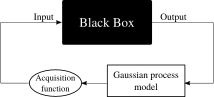
\includegraphics[width=8.4cm]{figs/bb_approach.pdf}
    \caption{Schematic illustration of \acrlong{bo}.}
    \label{fig:overview_bo}
\end{figure}
In \gls{bo} a \gls{gpm} is used to model the objective function.
The set of \(n\) observations is defined by \(\mathcal{O}=\left\{(\bx_k,y_k), k=1\dots n\right\}\) and is composed of the evaluated inputs combined with the corresponding observations. The compact notation of all inputs of \(\mathcal{O}\) is given by the matrix \(X = [\bx_{1}, \dots, \bx_{n}]\) and of all observations by the vector \(\bm{y}=[y_1,\dots,y_n]\). With the \gls{gpm}, the posterior distribution \(p(f_*\vert \mathcal{O},\bx_*,\bm{\theta})\) for \(f_* \widehat{=} f(\bx_*)\) at test point \(\bx_*\in\mathcal{X}\) is determined. Defining \([K(Z,Z')]_{(i,j)} = k(\bm{z}_i,\bm{z}'_j)\) where \(Z\in\mathbb{R}^{d\times m}\), \(Z'\in\mathbb{R}^{d\times k}\) and \(\bm{z}_i,\bm{z}'_j\in \mathbb{R}^d\), and substitute \(K=K(X,X)\), \(K_*=K(\bx_*,\bx_*)\), then, the posterior mean is defined as 
\begin{equation}
\begin{aligned}
    \mu(\bx_*) &= \mathbb{E}\left[p(f_*\vert \mathcal{O},\bx_*,\bm{\theta})\right] \\
                &= K(\bx_*,X)\left(K+\sigma_n^2I\right)^{-1}\bm{y}
\end{aligned}
    \label{eq:post_mean}
\end{equation} 
and the posterior variance as 
\begin{equation}
    \begin{aligned}
    \sigma^2(\bx_*) &= \mathrm{Var}\left[p(f_*\vert \mathcal{O},\bx_*,\bm{\theta})\right]\\
                    &=K_*-K(\bx_*,X)\left(K+\sigma_n^2I\right)^{-1}K(X,\bx_*).
    \end{aligned}
    \label{eq:post_var}
\end{equation}
Finally, the loop in \cref{fig:overview_bo} is closed by the acquisition function, which determines new promising inputs from the predictive distribution. A common choice is \gls{ei} as initially described in \cite{EI2} and \cite{EI}. This acquisition function determines the expectation that the function at point \(\bm{x}\) improves the so far best observation \(f_\mathrm{opt}\). 
\begin{align}
    \mathrm{EI}(\bm{x}) := \mathbb{E}\left[\max(f_\mathrm{opt}-f(\bm{x}),0)\right]
\end{align}   
For numerically evaluation we need to rewrite the expression into integral form. Using integration by parts gives
\begin{align}
    \mathrm{EI}(\bm{x}) = \left(f_\mathrm{opt}-\mu(\bm{x})\right)\cdot \Phi_s\left(\lambda\right) + \sigma(\bm{x})\cdot \phi_s \left(\lambda\right),
    \label{eq:ei}
\end{align}
where \(\lambda = \left(\frac{f_\mathrm{opt}-\mu(\bm{x})}{\sigma(\bm{x})}\right)\), \(\phi_s\) denotes the standard normal \gls{pdf} and \(\Phi_s\) represents the standard \gls{cdf}.
Two other widely used functions are \gls{ucb} \(u_i(\bm{x})\) and \gls{lcb} \(l_i(\bm{x})\) given by
\begin{equation}
\begin{aligned}
    u(\bm{x}) = \mu(\bm{x}) + \beta_i\sigma(\bm{x}),\\
    l(\bm{x}) = \mu(\bm{x}) - \beta_i\sigma(\bm{x}).
    \label{eq:ucb_lcb}
\end{aligned}
\end{equation}
The confidence \(\beta_i\) acts as trade-off between exploration and exploitation. Exploration means points with a high uncertainty are evaluated, whereas exploitation means that the function is optimized within a well known space. \gls{ucb} and \gls{lcb} are later especially used to define safe inputs as described in \cref{sec:safeBO}.

Using this naive \gls{bo} method we are facing several challenges for high-dimensional problems.
A very intuitive problem is the significantly increased number of evaluations to find the optimum. This can lead, depending on the required time for one evaluation, to prohibitively high run times. In addition, the computational complexity of inferring the posterior distribution is cubic to the number of observations due to matrix inversion. Another major limitation is seeking for new promising inputs with an acquisition function \(\alpha\). New inputs are defined by 
\begin{align}
    \bm{x}_\mathrm{new} = \argmax_{\bm{x} \in \mathcal{X}}\alpha(\bm{x}),
\end{align}
which corresponds to global optimization of a non-convex function across the whole input space. \cite{Moriconi2020} deems this operation is feasible up to problem dimension \(\dim(\mathcal{X}) = 10, \dots, 20\).

One approach to address the latter two issues is to divide the overall optimization problem into several sub-problems which are solved successively as shown in \cref{algo:ss_bayesopt}.
Initially, a direction oracle \(\Pi\) defines new directions \(r_i \in \mathrm{span}\{\mathcal{X}\}\). Commonly, a random oracle is utilized. Then, the subspace \(\mathcal{L}\) is constructed and \gls{bo} is applied on the subspace.
The optimization of \(\alpha\) can now be achieved via, \eg grid-based methods as \(\mathcal{L}\) is a low-dimensional space. In the following we refer to LineBO when \(\dim(\mathcal{L}) = 1\) (\cite{lineBO}) and to PlaneBO when \(\dim(\mathcal{L}) = 2\). 

\IncMargin{1.5em}
\begin{algorithm2e}[t]
 \DontPrintSemicolon
    \KwIn{direction oracle \(\Pi\),\newline initial point \(\bm{x}_0\),\newline parameter space \(\mathcal{X}\),\newline initial observation set \(\mathcal{O}_0 \),\newline GP prior \(G_0\) }
    \KwOut{\(\bm{x}_\mathrm{opt}\)}
    
    \For {\(i \leftarrow 1\) \KwTo \(M\)}{
    	\(r_i \leftarrow \Pi(G_{i-1})\) \tcp*[f]{determine next direction}\;
    	\(\mathcal{L}_i \leftarrow \{\bm{x}_{i-1}+\alpha \cdot r_i, \alpha \in \mathbb{R}\} \cap \mathcal{X}\)\;
    	\(\bm{x}_{i},\mathcal{O}_i, G_i \leftarrow \text{\gls{bo}}(\mathcal{O}_\mathrm{i-1},\mathcal{L}_i)\) \tcp*[r]{apply (safe)}
    	\tcp*[r]{\gls{bo}}
    }
    \(\bm{x}_\mathrm{opt} \leftarrow \bm{x}_{\mathrm{M}}\)
    \caption{Sequential Subspace \acrlong{bo} by \cite{lineBO} \label{algo:ss_bayesopt}}
\end{algorithm2e}

Another challenge deals with the definition of implicit constraints \(g:\mathcal{X} \longrightarrow \mathbb{R}\) on the input space. We define a constrained optimization problem as
\begin{align}
    \min_{\bm{x}\in\mathcal{X}} f(\bm{x}) \mathrm{\qquad s.\,t.\qquad} g(\bm{x})\leq 0.
\end{align}
One approach to include constraints is shown in \cite{safeopt1} and \cite{safeoptberkenkamp}. Based on these works, in \cref{sec:safeBO} a new algorithm is introduced.


%===============================================================================================================
\section{Modified Safe Bayesian Optimization} \label{sec:safeBO}
In the following, the safe \gls{bo} method introduced by \cite{safeoptberkenkamp}, SafeOpt, is formulated in terms of a minimization in order to present the differences of the algorithms proposed here. In SafeOpt, the input domain is divided into three subsets, the safe set \(\mathcal{S}\), the expander set \(\mathcal{G}\) and the minimizer set \(\mathcal{M}\). 
% The safe set is defined as 
% \begin{align*}
%     \mathcal{S} = \bigcup\limits_{\bx\in\mathcal{S}_\mathrm{prev}} \{\bm{x}'\in \mathcal{X}\lvert u(\bx)+Ld(\bm{x},\bm{x}') \leq T\},
% \end{align*}
% where \(T\) denotes the safety threshold, \(d(\bx,\bx')\) a distance measure between point \(\bx\) and \(\bx'\), \(\mathcal{S}_\mathrm{prev}\) the safe set of the previous iteration and \(L\) the Lipschitz constant of the target function. As this function is in a black box approach unknown a definition involving a Lipschitz constant is hardly realizable. 
The safe set is defined as
\begin{align}
    \mathcal{S} = \{\bm{x}\in \mathcal{X}\lvert u(\bx) \leq T\},
    \label{eq:safeset_berk}
\end{align}
 and depends on the \gls{ucb} as well as on the safety threshold \(T\) that should never be exceeded. The confidence of \gls{ucb} is given by
 \begin{align*}
    \beta = \left(2B+300\gamma_n\log^3\left(\frac{n}{\delta}\right)\right)^{1/2},
\end{align*} 
where \(B\) is a upper bound on the \gls{rkhs} norm of \(f\), \(\gamma_i\) the maximal mutual information obtained from the \gls{gpm} prior given \(n\) observations and \(\delta\) the allowed failure probability. Note that \(\beta\) is varying with iteration number or rather observation number, \cf \eqref{eq:ucb_lcb}; see \cite{safeopt1} for further details.
\cite{safeopt2} mention that this selection of the confidence may be too conservative. An alternative is to set \(\beta_i\) constant, \(\beta_i = \beta , \forall\, i\), as done in \cite{safeoptberkenkamp}. With respect to the expander set, \cite{safeoptberkenkamp} provide a formulation of it without using a Lipschitz constant. The indicator function given as
\begin{align}
    p(\bm{x}) = \lvert\{\bm{x}'\in \mathcal{X}\setminus \mathcal{S}\lvert u_{(\bm{x},l(\bm{x}))}(\bm{x}')\leq T\}\rvert
\end{align}
determines the number of additional safe set members by adding an artificial pair to the observation set, \((\bx, l_i(\bx)) \bigcup \mathcal{O}\). Then, after updating the posterior distribution, it is checked whether the safe set could be enlarged. If there is an expansion, \(\bx\) is added to the expander set which is defined as \(\mathcal{G}=\{\bx\in \mathcal{S}\vert p(\bx) > 0\}\).
Calculating the expander set with this formulation is very expensive as the posterior distribution needs to be recalculated for every member of the safe set. As shown in \eqref{eq:post_mean} and \eqref{eq:post_var} this involves a inversion of the matrix \(K\) which defines the covariance between the observations. As the observations change (an artificial pair is added) the matrix inversion need to be repeated.

%===============================================================================================================
\subsection{Algorithm}
\Cref{algo:modified_safeOpt} presents the modified safe optimization algorithm (MoSaOpt). The procedure consists of two different states which are entered successively without alternation, so if the algorithm once switches from exploration (which is always the initial state) to exploitation it can never enter exploration again. Due to the fact that \(f\) is completely unknown, there exists no information about the location of the minimum, hence, the reachable set, \(\mathcal{R} = \left\{\bm{x}\in \mathcal{X}\vert f(\bm{x})\leq T, \bx_0 \in \mathcal{S}_0\right\}\), must be observed. The reachable set is a compact subset of \(\mathcal{X}\) where the constraint is satisfied and depend on the start point \(\bx_0\). In the following, the constraint is assumed to impose an upper bound on the function value, such that 
\begin{align}
    g(\bx) = f(\bx) - T.
\end{align}
If \(g\) would be an independent function, an additional \gls{gpm} needs to be learned for \(g(\bx)\) as in \cite{safeBO3} and in \cite{heat_pump2}.
In order to initialize the algorithm, an initial safe set \(\mathcal{S}_0\) is required which consists of at least one point that satisfy the constraint. The initial set of observations \(\mathcal{O}_0\) can be empty, the confidence \(\beta\) is set constant and together with \(\bm{\theta }_0\) they are adjusted to fulfill the assumptions of Proposition~\ref{prop:1}. The output of the algorithm are the final set of observations and the optimal solution.
The optimization runs until a termination condition is fulfilled. Such a condition could be satisfied if the maximal value of the acquisition function \(\alpha\) falls below a threshold or if the maximal number of observations \(N\) is reached. Initially, the algorithm is in exploration state, where the safe set is defined in \linea{4} by the \gls{ucb}. The set of expanders is given as
\begin{align}
    \mathcal{G}_i = \partial\mathcal{S}_i
\end{align} 
and restricted to the boundary of the safe set, where the inputs with the greatest potential increase of \(\mathcal{S}\) are located. The new definition of expanders reduces the computational complexity significantly compared to the formulation in \cite{safeoptberkenkamp} as the boundary can be cheaply determined for one or two-dimensional spaces. Remind, that we assume the algorithm to be embedded into LineBO or PlaneBO. The exploration function in \linea{6}
\begin{align}
w(\bm{x}) = u(\bx) - l(\bx) = 2\beta\sigma(\bx)    
\end{align}
selects the expander with the highest uncertainty. Therefore, the expansion of \(\mathcal{S}\) is maximized and \(\mathcal{R}\) is observed within the least possible number of steps. These steps are repeated until the values of the exploration function falls below an exploration threshold \(\nu\) which indicates that the \(\nu\)-Reachable set \(\mathcal{R}_\nu \subset\mathcal{R}\) is observed. 

\IncMargin{0em}
\begin{algorithm2e}[t]
\DontPrintSemicolon
\KwIn{Initial safe set \(\mathcal{S}_0\),\newline acquisition function \(\alpha(\bm{x})\),\newline safety threshold \(T\),\newline confidence \(\beta\), \newline initial set of observations \(\mathcal{O}_0\), \newline initial hyperparameters \(\bm{\theta}_0\)}
\KwOut{\(\bm{x}_\mathrm{opt}\), \(\mathcal{O}\)}
\(\mathcal{G}_0 \leftarrow \partial\mathcal{S}_0\)\;
\(i \leftarrow 1\)\;
\While{termination condition not true}{
	\uIf(\tcp*[f] \textbf{exploration}){\(\nu \leq w_i(\bx), \bx\in\mathcal{G}_{i-1}\)}{
    \(\mathcal{S}_i \leftarrow \mathcal{S}_\mathrm{i-1} \bigcup \left\{\bm{x}\in \mathcal{X}\lvert u(\bm{x}) \leq T\right\}\)\;
    \(\mathcal{G}_i \leftarrow \partial\mathcal{S}_i\)\;
    %\(\mathcal{M}_i \leftarrow \left\{\bm{x}\in\mathcal{S}_i\lvert l(\bm{x}) \leq \min\limits_{i = 1:\lvert\mathcal{O}\rvert} (y_i)\right\}\)\;
		\(\bm{x}_i \leftarrow \argmax\limits_{\bm{x}\in \mathcal{G}_i} (w(\bm{x}))\)\;
	}
	\Else(\tcp*[f] \textbf{exploitation}){
	\(\bm{\theta}_i = \argmax\limits_{\bm{\theta}}\left(p(\bm{y}\vert X,\bm{\theta}_{i-1})\right)\)\;
    \(\mu_i(\bx_*) \leftarrow \mathbb{E}\left[p(f_*\vert \mathcal{O}_i,\bx_*,\bm{\theta}_i)\right]\)\;
    \(\sigma_i^2(\bx_*) \leftarrow \mathrm{Var}\left[p(f_*\vert \mathcal{O}_i,\bx_*,\bm{\theta}_i)\right]\)\;
   \(\mathcal{M}_i \leftarrow \left\{\bm{x}\in\mathcal{S}_i\lvert l(\bm{x}) \leq\Phi(\bm{y},X)\right\}\)\;
		\(\bm{x}_i \leftarrow \argmax\limits_{\bm{x}\in \mathcal{M}_i}(\alpha(\bm{x},\mu_i,\sigma_i))\)\;
	}
	\(y_i \leftarrow f(\bm{x}_i)+\epsilon\)\tcp*[f] evaluate function\;
	\(\mathcal{O}_i \leftarrow \mathcal{O}_{i-1} \bigcup \left\{\bm{x}_i,y_i\right\}\)\tcp*[f] update observation set\;
	\(i\leftarrow i+1\)\;
}
\(\bm{x}_\mathrm{opt} \leftarrow \arg\Phi(\bm{y},X)\) \tcp*[f] find optimal input\;
\caption{Modified Safe Optimization (MoSaOpt) \label{algo:modified_safeOpt}}
\end{algorithm2e}

If the uncertainty of the expanders falls below \(\nu\), the algorithm switches to exploitation state. The safe set is frozen and the hyperparameters are adjusted such that the marginal likelihood \(p(\bm{y}\vert X,\bm{\theta})\) becomes maximal. In this operation we are searching for a model that can explain the acquired data best with the lowest complexity as described in \cite{williams2006gaussian}. The model complexity means how fast the target function is assumed to vary. The higher the complexity of the model the more functions can be modeled. Then, in \linea{12} new promising inputs are selected from the optimized \gls{gpm} by the acquisition function \(\alpha\). In our implementation we use expected improvement \eqref{eq:ei} acquisition function. The inputs are from the minimizer set given as
\begin{align}
    \mathcal{M}_i = \left\{\bm{x}\in\mathcal{S}_i\lvert l(\bm{x}) \leq \Phi(\bm{y},X)\right\},
\end{align} 
Minimizers represents inputs that potentially improve the performance, here, indicated by a smaller \gls{lcb} than the current best observation determined by the decision function \(\Phi(\bm{y},X)\).
After that, \(f\) is evaluated at the obtained input in \linea{14} and the set of observations is updated. Finally, when the termination condition is fulfilled, the best solution of the observation set is identified by a decision scheme \(\arg\Phi(\bm{y},X)\) and returned.

The safety critical part of the optimization occurs in exploration state where the \(\nu\)-Reachable set is discovered. In order to guarantee safeness Proposition~\ref{prop:1} need to be fulfilled.
\begin{prop}
    Given \cref{assum:1}, constant \(\beta\) and that the initial hyperparameters \(\bm{\theta}_0\) as well as \(k(\cdot,\cdot)\) can be selected such that \(u(\bx)\geq f(\bx), \forall \bx \in \mathcal{X}\), then safeness is guaranteed by \cref{algo:modified_safeOpt} in the sense that \(f(\bx_i) \leq T, \forall \bx_i \in \mathcal{O}\).
\label{prop:1}
\end{prop}

\begin{proof}
    Follows directly from the definition of the safe set in \linea{3} of \cref{algo:modified_safeOpt}, evaluations are solely performed at \(\bx\in\mathcal{G}\bigcup\mathcal{M}\) where \(\left(\mathcal{G}\bigcup\mathcal{M}\right)\subset \mathcal{S}\).
\end{proof}
The length scales \(\bm{l}\) define how fast the covariance between neighbouring inputs decrease. The smaller the length scales, the faster the function values can change. The signal variance \(\sigma_f^2\) defines the range where the function values are expected. The larger \(\sigma_f^2\) the higher the expected range of function values. Adjusting these two hyperparamters realize the assumptions in Proposition~\ref{prop:1}, however, at the cost of convergence rate. Due to the scheme presented here, we can first explore the \(\nu\)-Reachable set while guaranteeing safety (see Proposition~\ref{prop:1}) and iteratively construct a data set containing information about the function in the \(\nu\)-Reachable set. Second, in exploitation safety is guaranteed since the safe set is no longer extended. We use the knowledge about the function given by the acquired data to perform a regression, \ie optimizing the hyperparamters. In practice, we obtain good approximations of the function (due to the conservatively chosen hyperparameters during exploration) such that the optimization of the function can be efficiently performed with only a few additional observations.  

%===============================================================================================================
\subsection{Practical Considerations}
The model complexity is adjusted by fitting the hyperparameters in \linea{8} via maximum likelihood estimation of the marginal likelihood \(p(\bm{y}\vert X,\bm{\theta})\). Since the marginal likelihood has several local optima one could end up at a bad local optimum with a very high complexity, \ie misinterpreting noise as function varies, if gradient based methods are applied. In general, the higher the dimension of the problem, the more local optima exist as the total number of hyperparameters is defined as \(\lvert\bm{\theta}\lvert = 2+d\); given by the \(d\) length scales (recall that \(d\) is the dimension of the input space \(d = \dim(\mathcal{X})\)), a signal variance and a noise variance. An intuitive approach is to apply gradient solvers from different start points, so different initial hyperparameters. Alternatively, instead of gradient solvers, one may apply global optimizers, \eg DIRECT as described in \cite{direct}. Here the problem dimension (number of hyperparameters) is the limiting factor. However, it would be sufficient to optimize the length scales of the considered subspace as observations in other dimensions have a minor influence due to the distance. For PlaneBO, the total number of hyperparameters to be optimized is then given as \(\lvert\bm{\theta}_\mathcal{L}\rvert = 4\), for which DIRECT is tractable. In our implementation, we decided to use a quasi-Newton method with dense Hessian approximation which shows in practice good results. However, with increasing dimension of the input space, restricting the optimization to the hyperparameters of the subspace can lead to better results. 

\begin{figure*}[htb]
    \centering
    \includegraphics[width = 0.9 \textwidth]{figs/lbsync21.pdf}
    \caption{Block diagram of the optical synchronization system for the simulation.}
    \label{fig:lbsync2}
\end{figure*}

The performance of sequential subspace optimizations rely significantly on the obtained input as following subspaces based on them (\cf \linea{3} in \cref{algo:ss_bayesopt}). The selection is performed in \linea{18} in \cref{algo:modified_safeOpt} using a decision function \(\Phi:\mathcal{O}\rightarrow \mathbb{R}\). A common approach is simply defining
\begin{align}
        \Phi(\bm{y},X)= \min_{i=1,\dots,n}(y_i).
        \label{eq:bad_descision_scheme}
\end{align}
However, recall that the observations are noisy as shown in \eqref{eq:y_composed}, the decisions made at the end of each subspace optimization would be prone to the measurement noise \(\bm{\epsilon}\), which invokes the occurrence of outliers. Outliers could be misinterpreted as good solutions and lead to a poor optimization as non optimal solutions are propagated to subsequent subspace optimizations.
Due to hyperparameter optimization, we decided to include the posterior mean of the fitted \gls{gpm} into the decision scheme \(\Phi(\bm{y},X)\) given as 
\begin{align}
    \Phi(\bm{y},X)=\min\limits_{\bm{x}_i, y_i\in \mathcal{O}}\big((1-\kappa)y_i+\kappa\mu(\bx_i)\big),
    \label{eq:new_decision_scheme}
\end{align}
where the posterior mean is weighted by a constant \(\kappa\) and the observations by \(1-\kappa\). The posterior mean is for a noise robust decision scheme quite useful as it is the solution of a regularization problem, given by the equivalent kernel 
\begin{align}
    J(f)= \frac{1}{2}\norm{f}_\mathcal{H}^2 + \frac{1}{2\sigma_n^2}\sum_i^n(y_i-f(x_i))^2.
    \label{eq:equivalent_kernel}
\end{align} 
Minimizing the equivalent kernel with respect to \(f\) lead to the posterior mean as in \eqref{eq:post_mean}; for further details see \cite{williams2006gaussian}.
The expression consists of two parts, \(\norm{f}_\mathcal{H}^2 \) represents the complexity and \(\sum_i^n(y_i-f(x_i))^2\) represents the accuracy, which is divided by the noise variance. This means that the weight of the accuracy term increases as the reliability on the observations does. Note that the complexity term depends on the \gls{rkhs} which is defined by the covariance function and its hyperparameters. As shown in \cite{williams2006gaussian}, optimizing the hyperparameters via maximum likelihood estimation will favour the least complex model that agrees with the data. Regarding \eqref{eq:equivalent_kernel}, this can be interpreted as increasing the weight on the complexity term (and decreasing the weight of the model fit as \(\sigma_n^2\) increases). This leads to a posterior mean that may not agrees completely with every data point but rejects small, fast variations which are invoked by noise. Depending on the noise level, \(\kappa\) can be used to define the trade-off. 


%=====================================================================================================
\section{Results} \label{sec:results}
In this section the algorithm presented here is compared to other safe \gls{bo} schemes; first in a simulation environment of the \gls{xfel} optical synchronization system and, second, at a small-scale laboratory optical synchronization system.

\subsection{Simulation Results} \label{subsec:comp}
The algorithm presented in \cref{sec:safeBO} is demonstrated in a simulation environment of the \gls{xfel} optical synchronization system as illustrated in \cref{fig:lbsync2}.
The system consists of \(N=5\) subsystems interconnected in a chain, each equipped with a \gls{pi} controller. The odd numbers corresponds to lasers and the even numbers to links. The reference signal \(r\) is white Gaussian noise colorized with the filter \(F_\mathrm{r}\). The disturbances \(d_1,\dots,d_\mathrm{N}\) are colorized white Gaussian noise respectively. The performance quantity is the integrated timing jitter \(J\) given by the \gls{rms} norm of the performance channel \(z\). Using the fact that the input signals are \gls{awgn} with \gls{psd} \(S(\omega) = 1\), following from Parseval's theorem the optimization corresponds to a \(\mathcal{H}_2\) minimization of the closed loop transfer function \(G_\mathrm{cl}(s)\) as shown in \cite{heuer}.
In the following we compare the algorithm presented in this work, MoSaOpt of \cref{algo:modified_safeOpt}, with SafeOpt from \cite{safeoptberkenkamp}. The goal is to find optimal PI-parameters. For \(N=5\), there are in total ten tuning knobs \(\mathcal{X}\subseteq \mathbb{R}^{10}\). In addition, we want to investigate the impact of the dimension of the subspace on the performance.
Therefore, we consider in total four \gls{bo} implementations:
\begin{enumerate}
\item LineBO + SafeOpt
\item LineBO + MoSaOpt
\item PlaneBO + SafeOpt
\item PlaneBO + MoSaOpt
\end{enumerate}

We use the Mat\'ern kernel with \(\nu = 3/2\), all initial hyperparameters are for each implementation chosen equivalently. We consider first a noise-free simulation, so the noise standard deviation is set to a very small value, \(\sigma_n = 10^{-5}\). In all trials we use expected improvement acquisition function, \(\alpha(\bx) = \mathrm{EI}(\bx)\). In addition, the maximum number of subspace iterations is restricted to \(M=40\) for LineBO and \(M=20\) for PlaneBO, because PlaneBO takes within one subspace optimization considerably more observations. As the set observations increases over the subspace optimizations, we run into risk of prohibitively high computational demand. Therefore, the combinations are restricted to the five PI-gains of each subsystem as well as the combinations of the P-gains of the laser subsystems resulting in
\begin{align*}
    r_i \in \bigg\{[P_1,P_3];[P_1,P_5];[P_3,P_5];[P_1,I_1];\dots;[P_5,I_5]\bigg\}.
\end{align*}
Recall that \(r_i\) is the direction selected in \linea{2} of \cref{algo:ss_bayesopt} by the direction oracle.
Here, we use a random oracle \(\Pi\) which selects the direction based on a uniform probability distribution over all possible subspaces. 
%As the random oracle is used, this restriction reduces the vulnerability to choose non effective subspaces and increases the comparability. Non-effective subspaces does not influence the value of the function and need not to be optimized. During the optimization, the I-gains of the laser subsystems could be identified as non effective spaces. However, in most applications, it is not possible to distinguish between effective and non-effective subspaces before the optimization. 
In order to provide a statistical evident comparison, the optimization of each method is ten times repeated for different start points.

\Cref{fig:bo_comparison} shows the results of the \gls{bo} comparison, it can be seen that line searches performs significantly better in terms of convergence rates, whereas PlaneBO + MoSaOpt provides a slightly improved solution quality. It is obvious that the \gls{bo} methods with MoSaOpt clearly improves robustness to different starting points as indicated by the smaller, covered, areas in \cref{fig:bo_comparison}. Furthermore, the new method improves the convergence rates for both implementations significantly. In case of LineBO with MoSaOpt, the variance could be reduced to its final value after only 217 observations and the optimum was found after 342 evaluations. In contrast, SafeOpt requires 432 and 671 observations respectively, which means that the number of evaluations is almost doubled. As expected, PlaneBO needs considerably more evaluations due to longer exploration. This results for the underlying system in a worse convergence rate; PlaneBO + MoSaOpt finds the optimum after 1365 evaluations as PlaneBO + SafeOpt required 2284. The high iteration numbers are cut in \cref{fig:bo_comparison}, due to illustrative reasons. However, \cref{fig:bo_comparison} shows, that PlaneBO + MoSaOpt converges significantly faster. 

\begin{figure}
    \centering
    \includegraphics[width = 8.4cm]{figs/Bo_Comparison.pdf}
    \caption{Comparison of the \gls{bo} methods based on the simulated system. The colored area corresponds to the single standard deviation and \ding{83} denotes the occurrence of the optimum.}
    \label{fig:bo_comparison}
\end{figure}

Furthermore,  we want to test the decision scheme \cref{algo:modified_safeOpt} \linea{18} in terms of robustness to noisy observations. Therefore, we run two optimizations with LineBO + MoSaOpt, one with the new decision scheme as in \eqref{eq:new_decision_scheme} with \(\kappa=0.9\) and one with the old decision scheme as in \eqref{eq:bad_descision_scheme}(equivalently to \eqref{eq:new_decision_scheme} if \(\kappa = 0\)). In addition, a noise term \(\epsilon \sim \mathcal{N}(0,2)\) is added to the output of the simulated plant. To compare the outcomes of both optimizations, the obtained optimal inputs are evaluated without noise. For \(\kappa = 0.9\) the mean optimal jitter is \(\bar{y}_{\mathrm{opt},0.9}=13.64 \)\,\si{fs}, whereas with \(\kappa=0\), \(\bar{y}_{\mathrm{opt},0.0}=15.78 \)\,\si{\femto\second}. Compared to the overall best solution found in the noise free case, we improve the solution about
\begin{align}
    \zeta_\mathrm{noise} = \frac{15.78-13.64}{12.18} \equalhat 17.61\%
\end{align}
when using the new decision scheme with a reasonable \(\kappa\).

\subsection{Experimental Results} \label{subsec:tuning}
In the following we present experimental results from a laboratory optical synchronization system at \gls{desy}. The considered chain, see \cref{fig:lbsync2}, has \(N = 2 \) components. An additional laser provides the reference signal but is not considered in the optimization. In this case, system 1 is the link and system 2 is the laser. The quantity of synchronization is again the integrated timing jitter \(J\) between the reference laser and the laser system 2 determined every \SI{0.1}{\second} by an out-of-loop \gls{oxc} denoted by the last, right summation in \cref{fig:lbsync2}. Advantages of this measurement device are a high resolution and a low noise level, thus we decided to set \(\kappa = 0.3\). However, the noise is further reduced by averaging over several jitter samples. In the first experiment 10 samples are used which corresponds to an expenditure of time of one second per jitter generation. In the second trial, the sample size is increased to 100. Each optimization is again repeated ten times for different start points. Now we compare LineBO + MoSaOpt with the well known Nelder-Mead algorithm as described in \cite{nelder_mead}. Additionally, two differnt oracles are used, namely random and descent as described in \cite{lineBO}. The descent oracle increases the local convergence rate, whereas with random oracle, also global guarantees are provided.   

\begin{figure}[tb]
	\centering
  \subfloat[One second jitter generation.]{
  \includegraphics{figs/comp_1sec.pdf}
  \label{fig:lab_comp1sec}
  }%
  \\
  \subfloat[Ten seconds jitter generation.]{
  \includegraphics{figs/comp_10sec.pdf}
  \label{fig:lab_comp10sec}
  }
  \caption{Performance comparison of LineBO + MoSaOpt with random and descent oracle, and Nelder-Mead based on a small-scale optical synchronization system consisting of a laser and a link.}
  \label{fig:lab_comparison}
\end{figure}

\Cref{fig:lab_comparison} illustrates the mean optimal jitter for ten different start points. The final, optimal performance of the LineBO implementations is equivalent, whereas using the descent oracle lead to a significantly improved convergence rate.  As expected Nelder-Mead shows a high convergence rate for the low dimensional problem, but is partially unable to find reasonable optima as shown in \cref{fig:lab_comp1sec}. This shows the low robustness of Nelder-Mead against noisy observations, even though the noise is small due to the high performance measurement device. In contrast, both \gls{bo} implementations show robust solutions against the start points and noise. Increasing the set of samples per jitter generation would clearly decrease the sample mean variance. As shown in \cref{fig:lab_comp10sec}, Nelder-Mead provides good solutions by averaging the jitter over 100 measurements, whereas this increases the time for averaging by a factor of ten to ten seconds. Comparing the optimization time of Nelder-Mead in \cref{fig:lab_comp10sec} and LineBO in \cref{fig:lab_comp1sec}, Nelder-Mead needs with approximately \SI{400}{\second}, five times longer than the LineBO implementations, which require \SI{80}{\second}. However, the solution qualities are equivalent in the sense that the obtained optima have the same performance. Considering time efficiency and solution quality LineBO + MoSaOpt clearly outperforms Nelder-Mead. Using the descent oracle increases the convergence rate significantly, whereas with random the optimal jitter is partially constant as shown in \cref{fig:lab_comp10sec}. This indicates that a subspace does not influence the synchronization or is already optimized. The descent oracle does not select such none-effective subspaces which results in a better convergence rate.  

%===============================================================================================================
\section{Conclusion} \label{sec:conclusion}
We presented a practical formulation of safe \acrlong{bo} (MoSaOpt) by separating exploration and exploitation combined with hyperparameter optimization. With this we can show in practice a significantly improved convergence rate while guaranteeing safety. In addition, hyperparameter optimization opens the applicability of a new, noise robust decision scheme which shows significantly better estimations of the true optimal value given noisy observations. This characteristic is especially decisive for sequential subspace optimization approaches, as wrong decisions would decrease the quality of the optimization process considerably. Furthermore, we demonstrated the performance of MoSaOpt on a simulated plant compared to an other safe \gls{bo} scheme. Experimental results on a physical plant showed the noise robustness in a comparison to a classical optimization algorithm like Nelder-Mead. 

\bibliography{biblio}
\end{document}